% !TeX encoding = UTF-8
\documentclass[aspectratio=169]{beamer}
\useoutertheme[progressbar=frametitle]{metropolis}
\useinnertheme{metropolis}
\definecolor{nabgray}{rgb}{0.6,0.59,0.61}
\usecolortheme[named=nabgray]{structure}

\usepackage{tikz}
\usepackage[utf8]{inputenc}
\usepackage[portuguese]{babel}
\usepackage{fontspec}
\setmonofont{JetBrains Mono}
\setmainfont{Roboto}
\setsansfont{Roboto}

\usepackage{smartdiagram}
\usepackage{qtree}
\usepackage{verbatim}
\usepackage{svg}
\usepackage{graphicx}
\usepackage{color}

\definecolor{lightgray}{rgb}{0.95, 0.95, 0.95}
\definecolor{darkgray}{rgb}{0.4, 0.4, 0.4}
%\definecolor{purple}{rgb}{0.65, 0.12, 0.82}
\definecolor{editorGray}{rgb}{0.95, 0.95, 0.95}
\definecolor{editorOcher}{rgb}{1, 0.5, 0} % #FF7F00 -> rgb(239, 169, 0)
\definecolor{editorGreen}{rgb}{0, 0.5, 0} % #007C00 -> rgb(0, 124, 0)
\definecolor{orange}{rgb}{1,0.45,0.13}
\definecolor{olive}{rgb}{0.17,0.59,0.20}
\definecolor{brown}{rgb}{0.69,0.31,0.31}
\definecolor{purple}{rgb}{0.38,0.18,0.81}
\definecolor{lightblue}{rgb}{0.1,0.57,0.7}
\definecolor{lightred}{rgb}{1,0.4,0.5}
\usepackage{upquote}
\usepackage{listings}
\lstset{language=java,
	basicstyle=\footnotesize\ttfamily,
	keywordstyle=\footnotesize\color{blue}\ttfamily,
	escapeinside={<@}{@>}
}


\usebackgroundtemplate%
{%
	
\includegraphics[width=\paperwidth]{Images/Contenido}%
}


\title{Design Patterns para Microsserviços com MicroProfile}
\author{Víctor Orozco}
\institute{Nabenik}
\date{\today}

\begin{document}
{
    \usebackgroundtemplate{
\includegraphics[width=\paperwidth]{Images/portada}}
    \setbeamercolor{frametitle}{fg=red}
    \usebeamercolor[fg]{normal text}
    \frame{\titlepage}
}


{
    \usebackgroundtemplate{
\includegraphics[width=\paperwidth]{Images/separador}}
    \setbeamercolor{normal text}{fg=white}
    \setbeamercolor{frametitle}{fg=red}
    \usebeamercolor[fg]{normal text}
    \section{Design Patterns}
}

\begin{frame}{Microserviçõs = Metapadrão arquitetural}


Arquitetura que estrutura o aplicativo como um conjunto de \textbf{serviços colaborativos fracamente acoplados}. Esta abordagem corresponde ao eixo Y do \textit{scale cube}. O objetivo final são \textbf{sistemas reativos}.

\begin{figure}
	\centering
	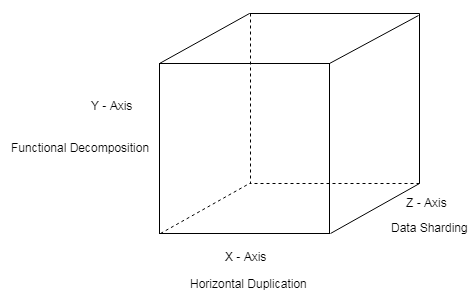
\includegraphics[width=0.7\linewidth]{Images/scale}
\end{figure}

\end{frame}

\begin{frame}{}

\begin{figure}
	\centering
	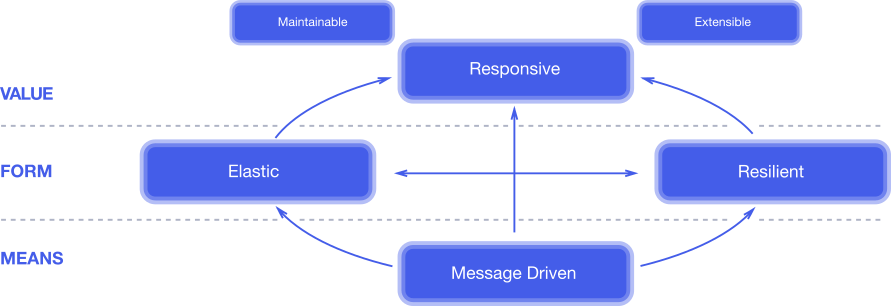
\includegraphics[width=\linewidth]{Images/reactive-traits.png}
\end{figure}

\end{frame}


\begin{frame}{Application Server}

	\begin{itemize}
		\item Transacionalidade distribuída (JTA/XA)
		\item Contratos (JNDI)
        \item Service discovery (JNDI)
        \item Deployment (EAR/Class Loaders/Dashboards)
		\item Métricas (JMX)
        \item Segurança (SoteriaRI/JACC)
	\end{itemize}

\end{frame}



\begin{frame}{Microserviçõs}

    Aplicativos Cloud Native
	\begin{itemize}
		\item Sistemas reativos
		\item 12 fatores Cloud Native
        \item Design patterns
        \item Domain Driven Design
		\item Microservice chassis e/ou service mesh
        \item Orquestração de contêineres
	\end{itemize}

\end{frame}


\begin{frame}{Microserviçõs = Metapadrão arquitetural}

    Cloud Native
	\begin{itemize}
		\item (Gostamos de ter) Sistemas reativos
		\item (É possível com a metodologia dos) 12 fatores Cloud Native
        \item (Usamos soluções testadas chamadas de) design patterns
        \item (Fragmentamos o sistema mediante) Domain Driven Design
		\item \textbf{(Implementamos os serviços com frameworks) microservice chassis e/ou service mesh}
        \item (E fazemos deployment) mediante orquestração de contêineres
	\end{itemize}

    Os Dessign Patterns são uma linguagem comum para \textit{implementar e avaliar plataformas Cloud Native}.

\end{frame}


\begin{frame}{}
\begin{figure}
	\centering
	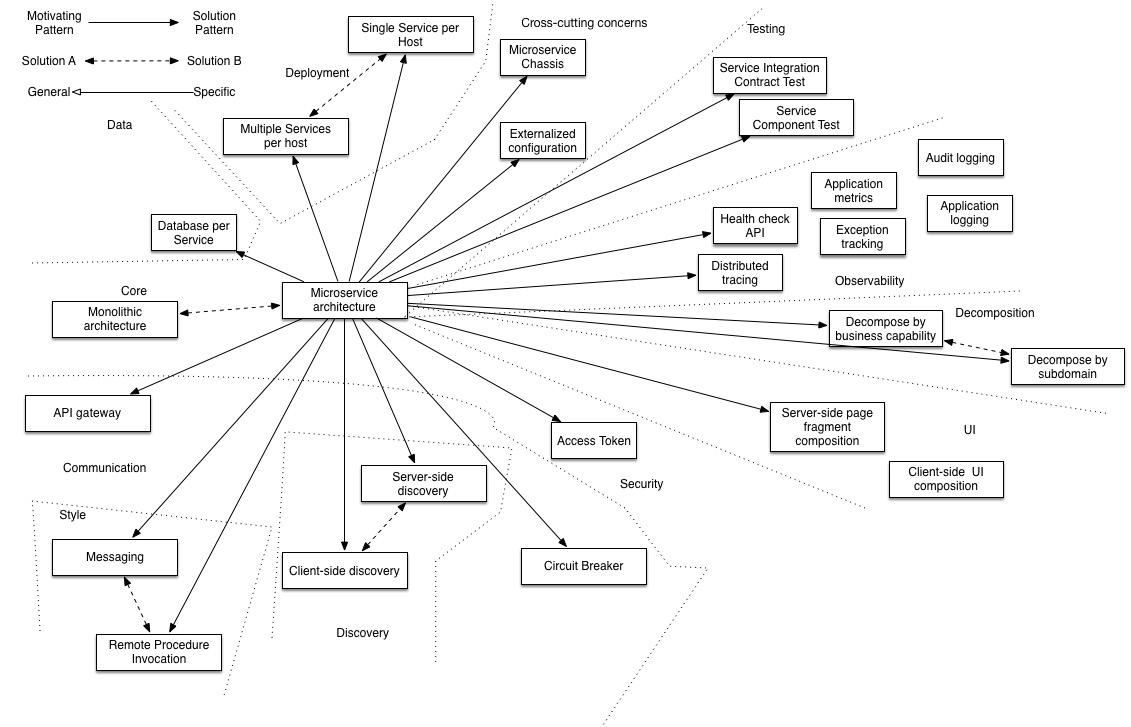
\includegraphics[width=\linewidth]{Images/PatternsRelatedToMicroservices}
\end{figure}
\end{frame}

\begin{frame}{}
\begin{figure}
	\centering
	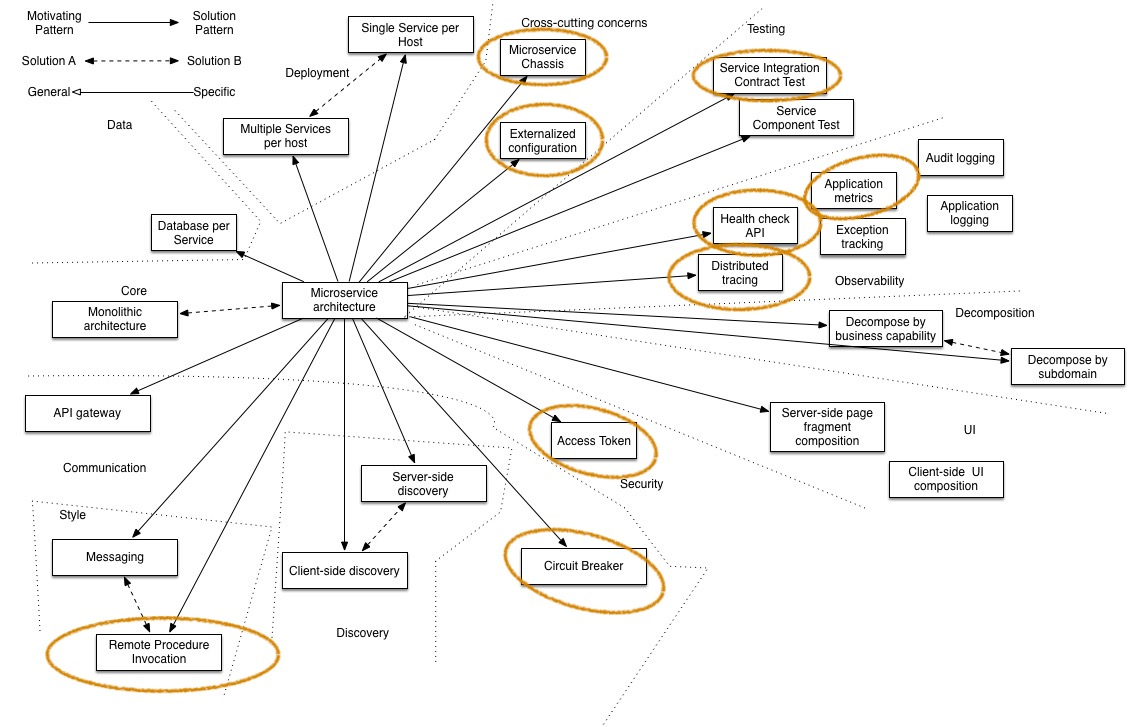
\includegraphics[width=\linewidth]{Images/PatternsRelatedToMicroservices2}
\end{figure}
\end{frame}



{
    \usebackgroundtemplate{
\includegraphics[width=\paperwidth]{Images/separador}}
    \setbeamercolor{normal text}{fg=white}
    \setbeamercolor{frametitle}{fg=red}
    \usebeamercolor[fg]{normal text}
    \section{MicroProfile}
}

\begin{frame}{A historia}
Os \textit{patterns} foram criados antes/junto com os chassis e antes do service mesh/K8S
\begin{figure}
	\centering
	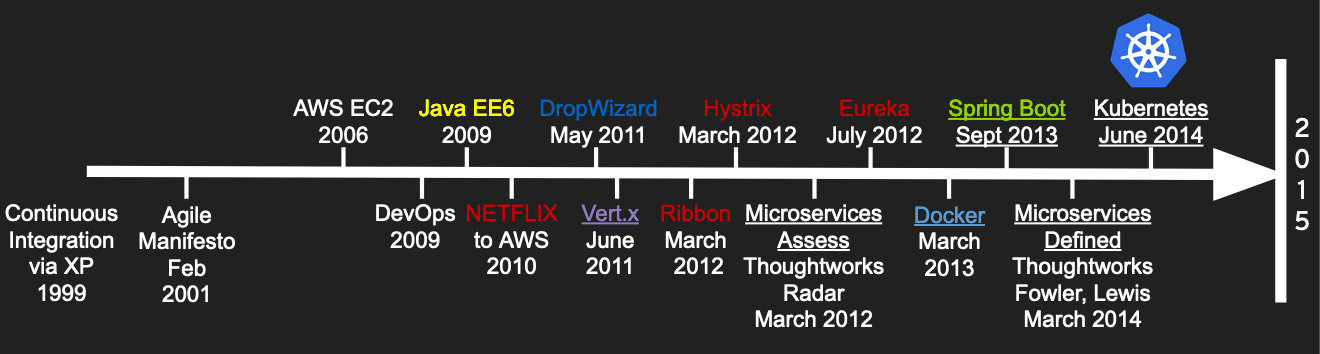
\includegraphics[width=\linewidth]{Images/timeline}
\end{figure}
Créditos: Rafael Benevides

\end{frame}


\begin{frame}{MicroProfile}



\begin{columns}[T] % contents are top vertically aligned
\begin{column}[T]{6cm} % each column can also be its own environment
	\begin{block}{Chassis}
No ponto de vista dos design patterns. Os frameworks "cloud native" são soluções para problemas "cross-cuting concerns".
	\end{block}
    \begin{block}{Chassis EE}
O MicroProfile é uma especificação para chassis fundamentada no Java/Jakarta EE
	\end{block}
\end{column}
\begin{column}[T]{7cm} % alternative top-align that's better for graphics
    \begin{figure}
    	\centering
    	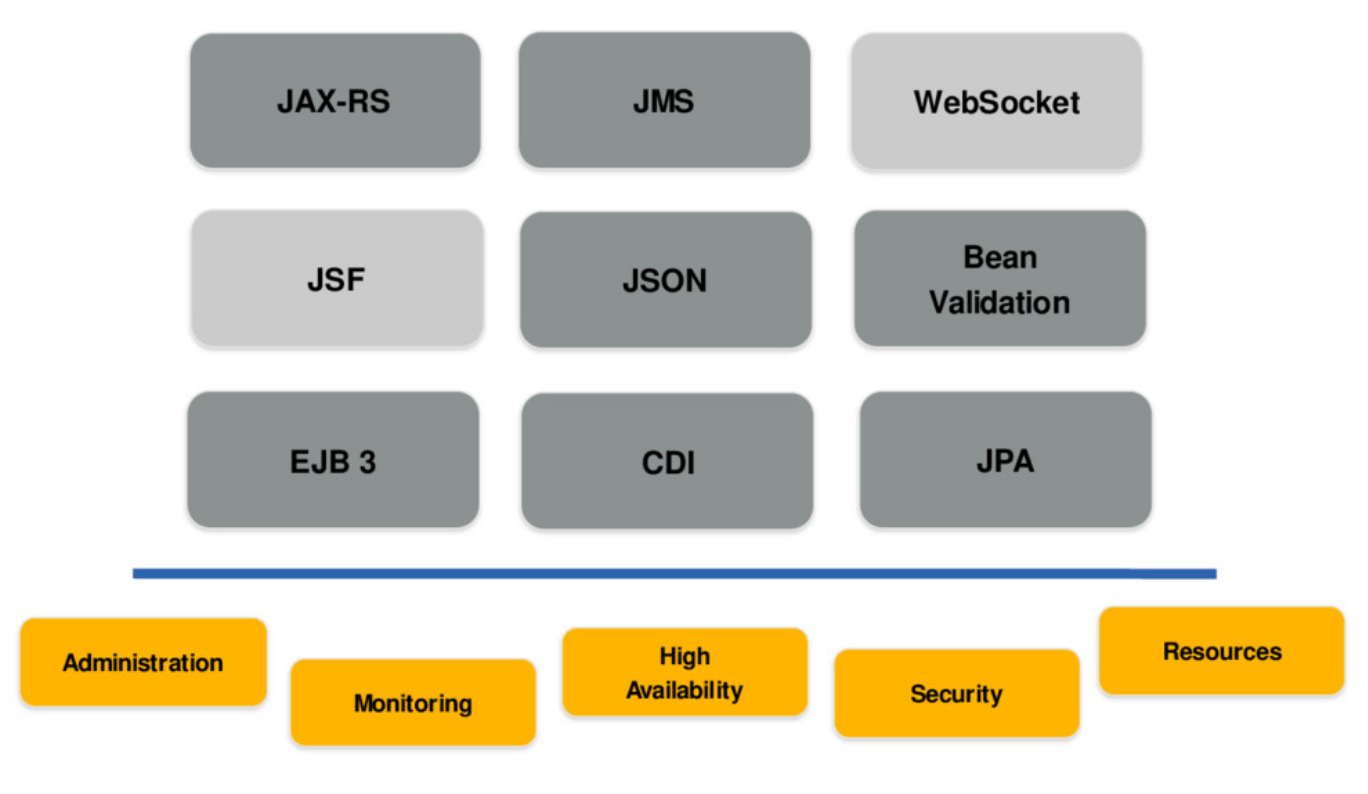
\includegraphics[width=\linewidth]{Images/javaeemicropancake}
    	\caption{Créditos: Reza Rahman}
    \end{figure}

\end{column}
\end{columns}

\end{frame}

\begin{frame}{MicroProfile}
\begin{figure}
	\centering
	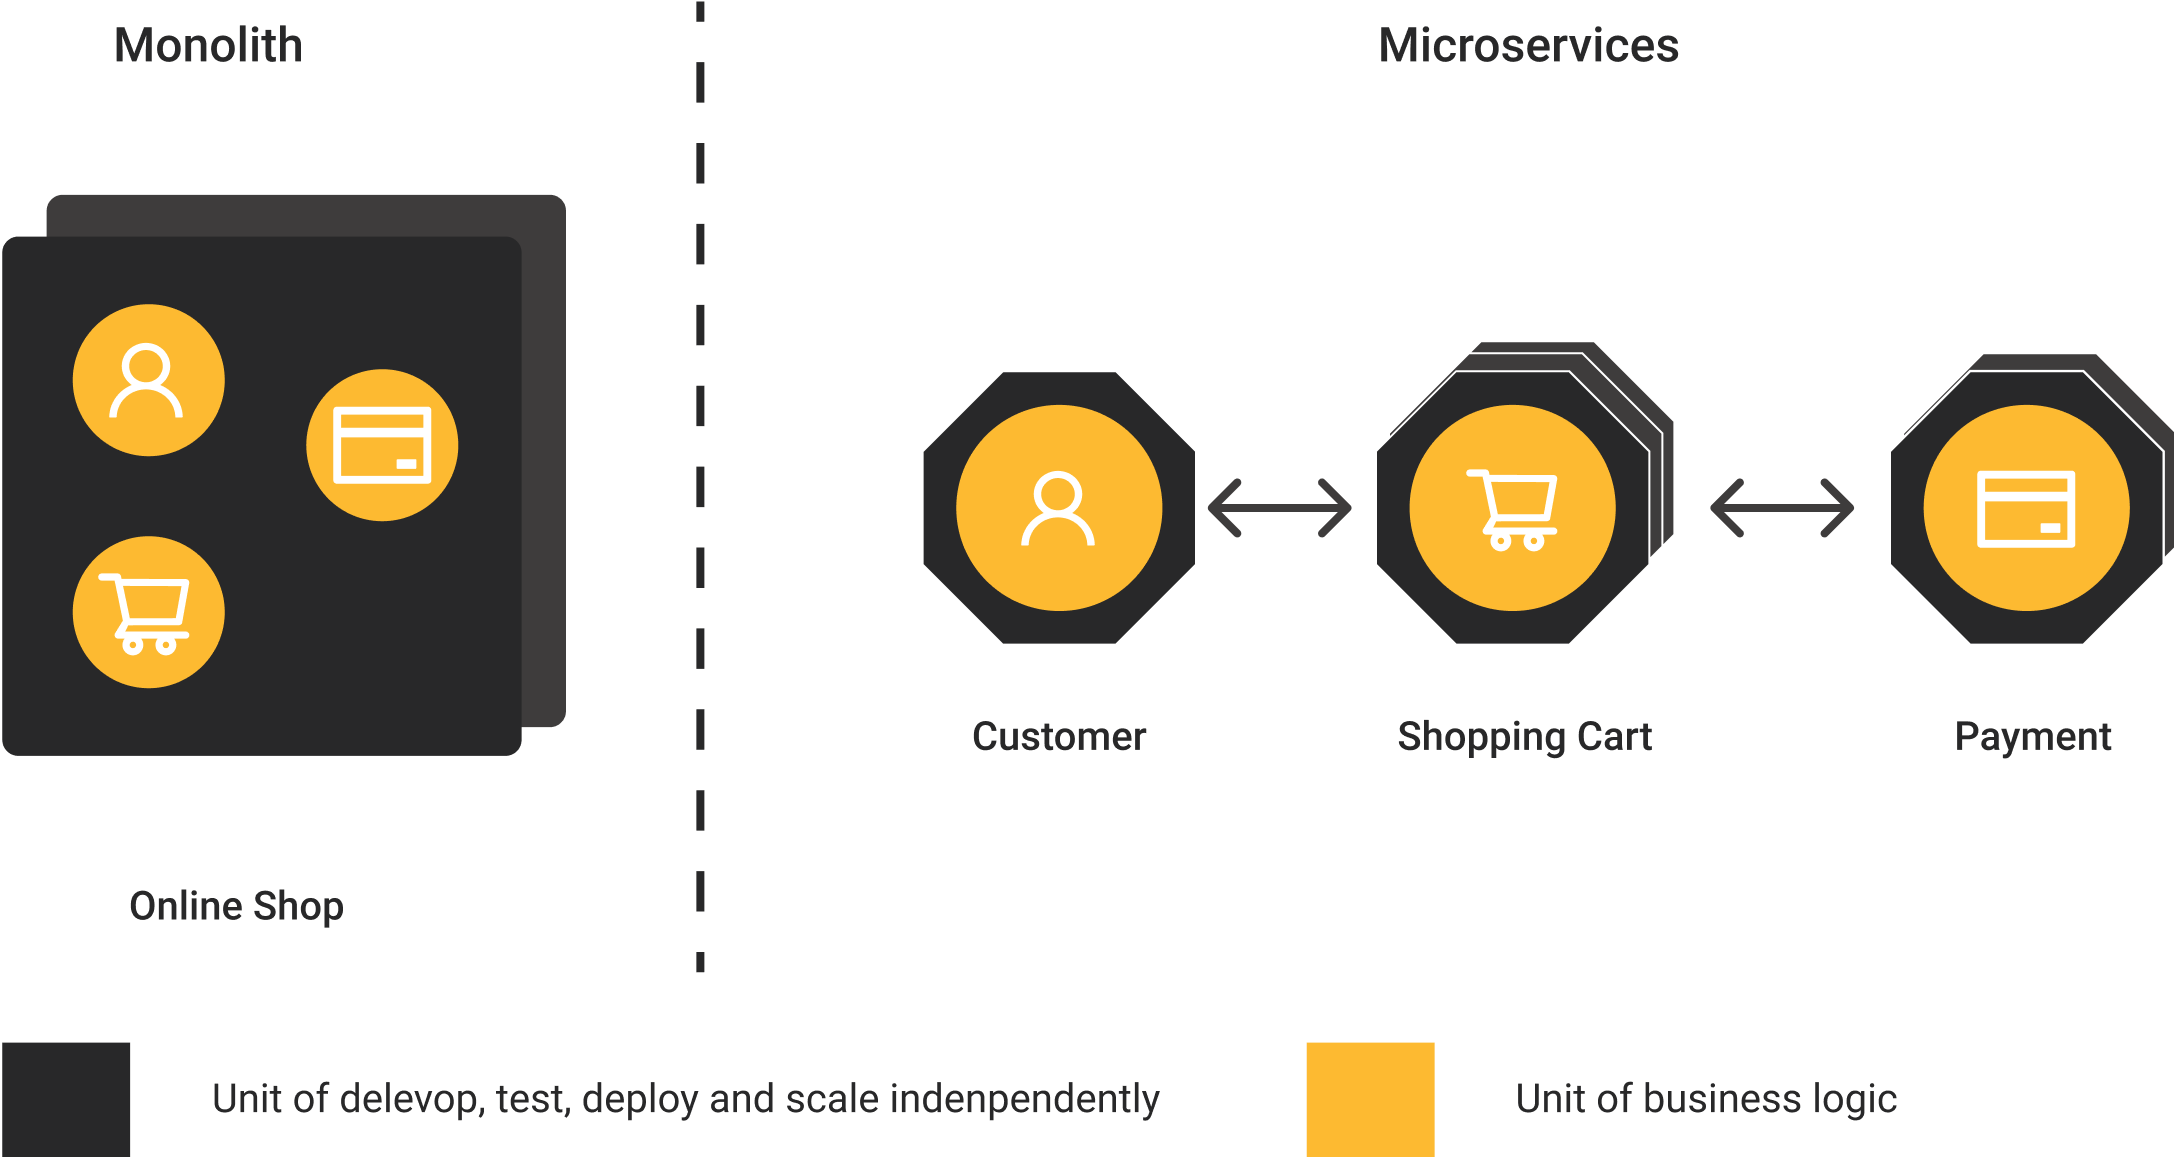
\includegraphics[width=0.7\linewidth]{Images/mp0}
\end{figure}
\end{frame}

\begin{frame}{MicroProfile - Coreografia}
Patterns complementarios - Event Sourcing, CQRS
\begin{figure}
	\centering
	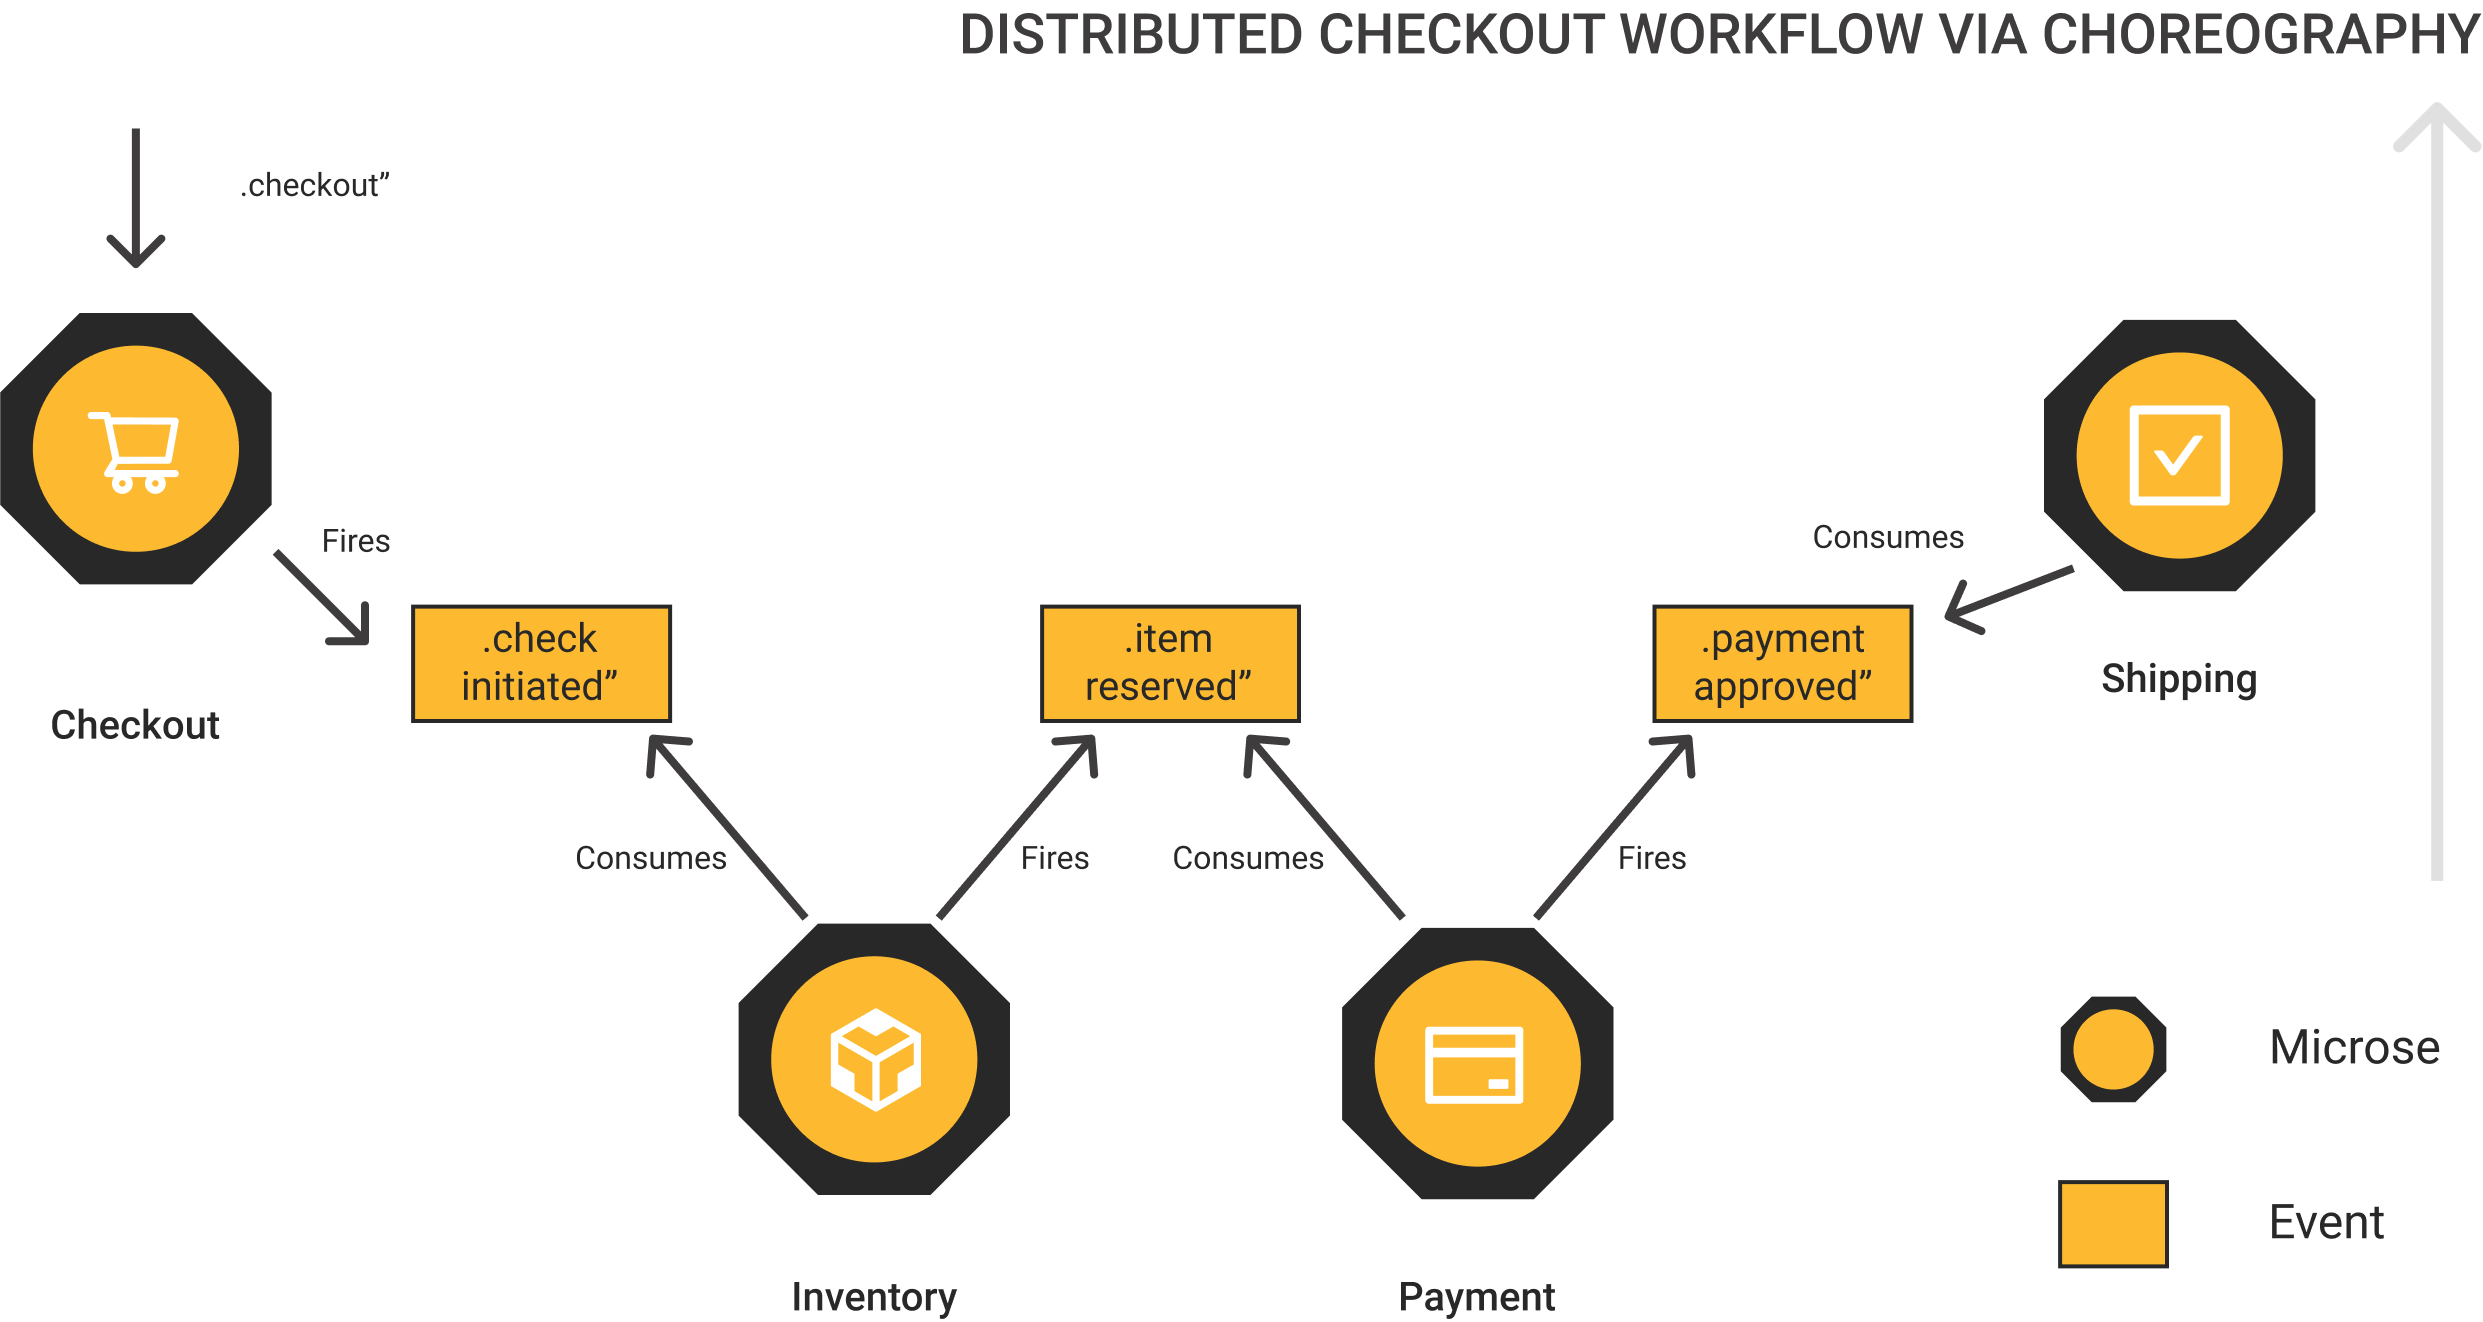
\includegraphics[width=0.7\linewidth]{Images/mpcore}
\end{figure}
\end{frame}

\begin{frame}{MicroProfile - Orquestador}
Patterns complementarios - SAGA
\begin{figure}
	\centering
	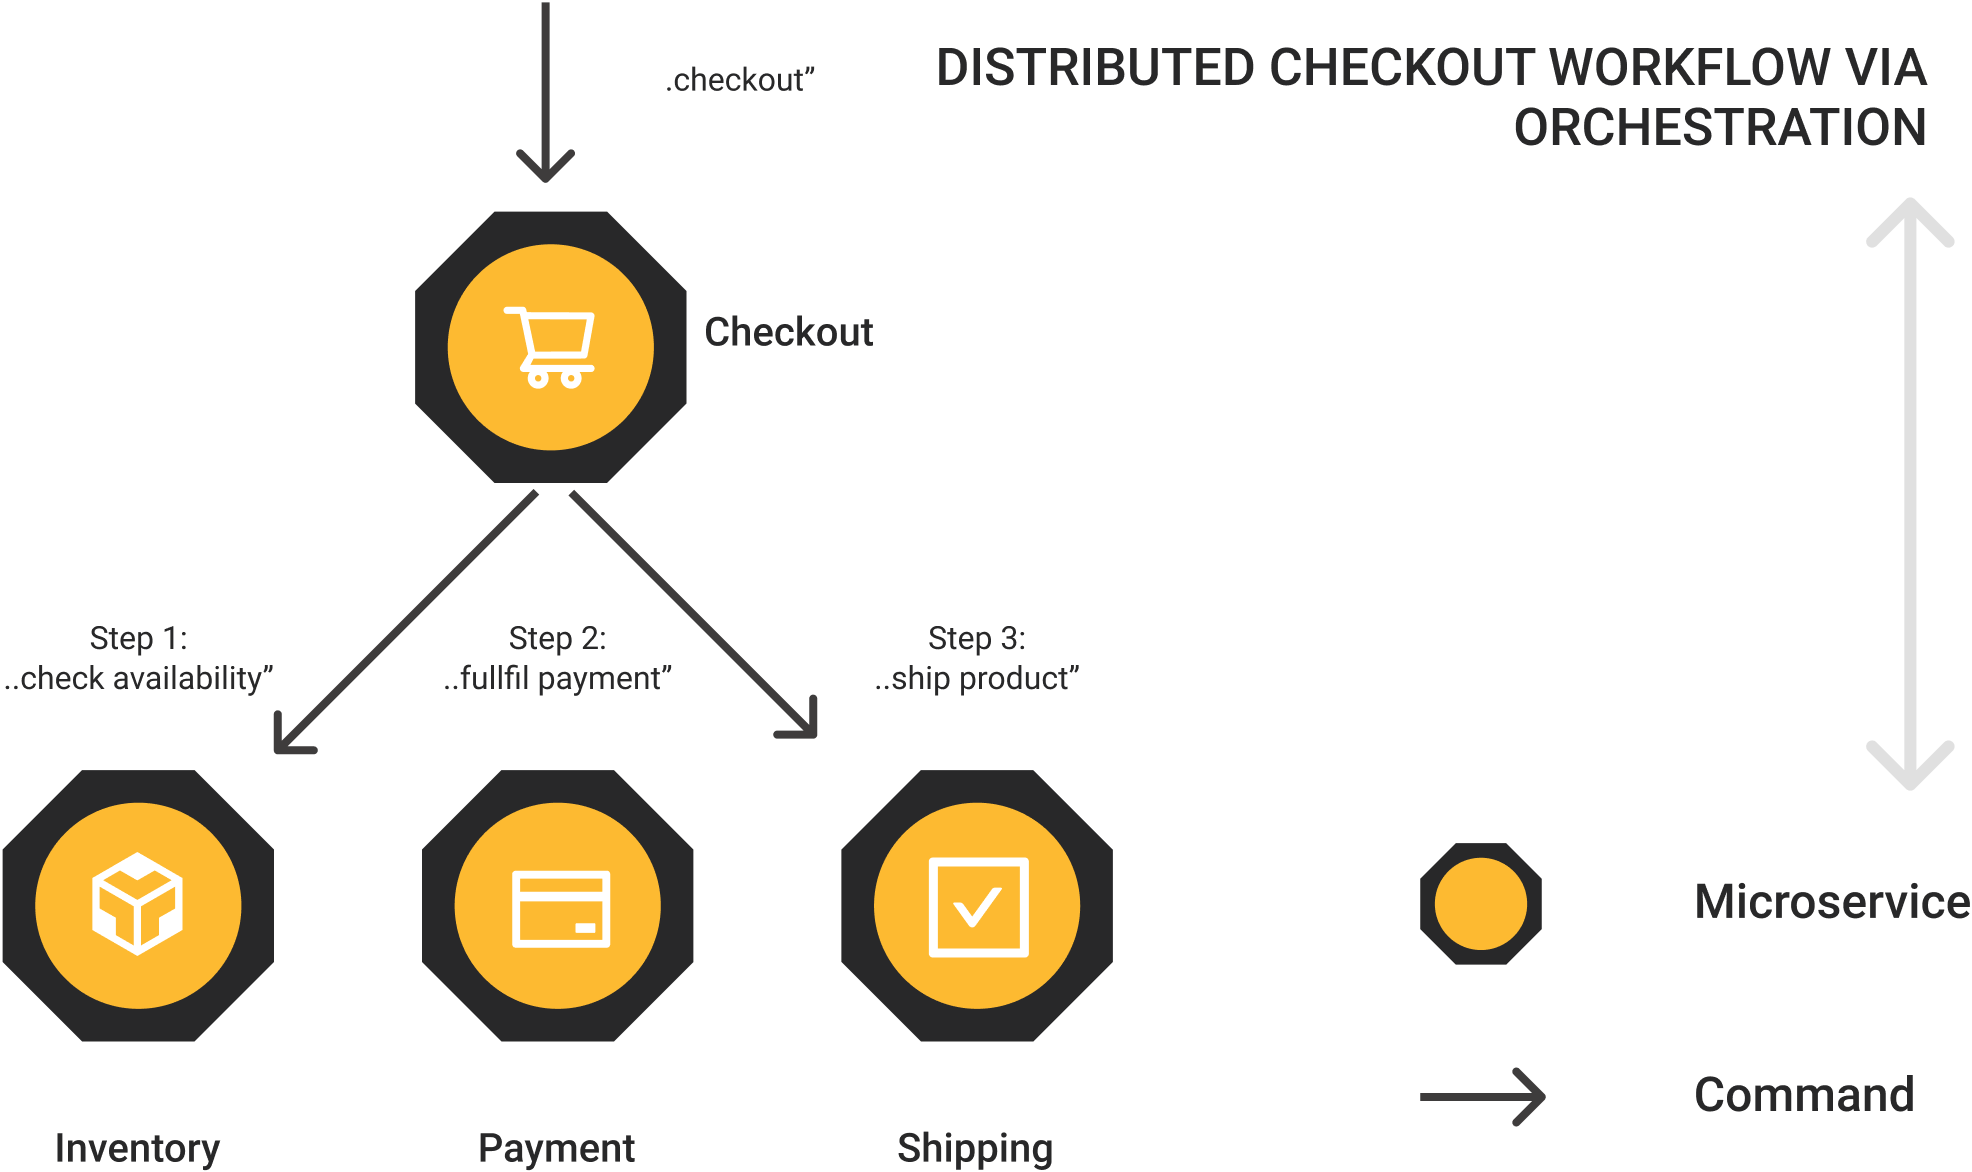
\includegraphics[width=0.7\linewidth]{Images/mporch}
\end{figure}

\end{frame}

\begin{frame}{Cross-cutting concerns no mundo real}

\begin{itemize}
	\item \textbf{Health checks \& Metrics} - Coletar metricas (Prometheus/Grafana) e estabelecer regras no deployment
	\item \textbf{Resilence \& Fault Tolerance} - Sobreposição entre service Mesh -e.g. Likerd, Istio- e MicroProfile Fault Tolerance
	\item \textbf{Configuration} - Injeção de configuração no ambiente
	\item \textbf{Authentication \& Authorization} - API Gateway + MicroProfile JWT
	\item \textbf{Standarized documentation} - OpenAPI + Swagger Server
    \item \textbf{Tracing} - MicroProfile Tracing + Zipkin
    \item\textbf{ Remote Procedure \& Messaging} - JAX-RS + MicroProfile Rest Client + K8S service discovery
\end{itemize}

\end{frame}


{
    \usebackgroundtemplate{
\includegraphics[width=\paperwidth]{Images/separador}}
    \setbeamercolor{normal text}{fg=white}
    \setbeamercolor{frametitle}{fg=red}
    \usebeamercolor[fg]{normal text}
    \section{MicroProfile - APIs}
}

\begin{frame}{EE + MicroProfile  - Demo}
Oracle Helidon (Chassis) +  Oracle Kubernetes Engine

\begin{itemize}
	\item Configuração
	\item Contrato e cliente REST
	\item Resiliência
	\item Deployment
	\item Health Check
    \item Metricas
\end{itemize}

\end{frame}

\begin{frame}{Config}
\begin{figure}
	\centering
	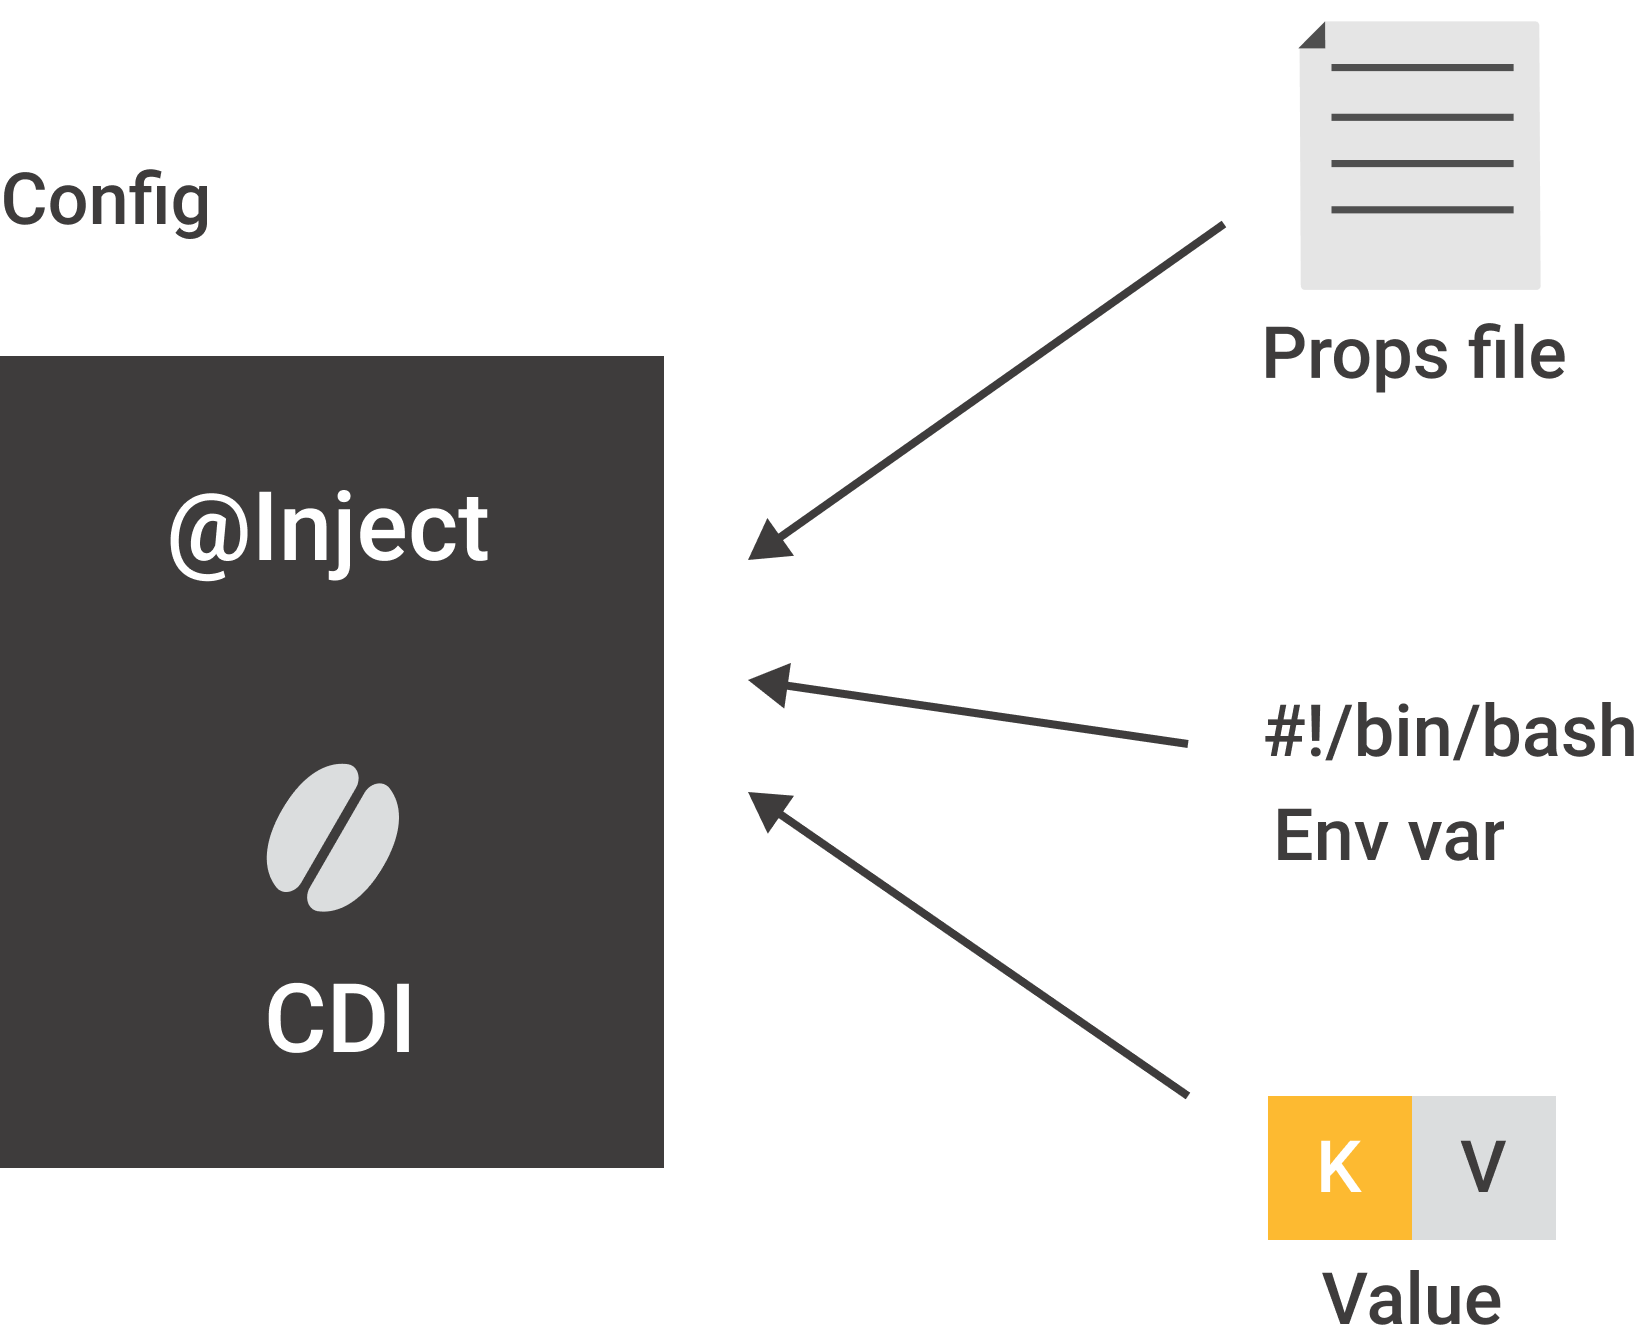
\includegraphics[width=0.65\linewidth]{Images/config}
\end{figure}
\end{frame}

\begin{frame}{Config}
\begin{figure}
	\centering
	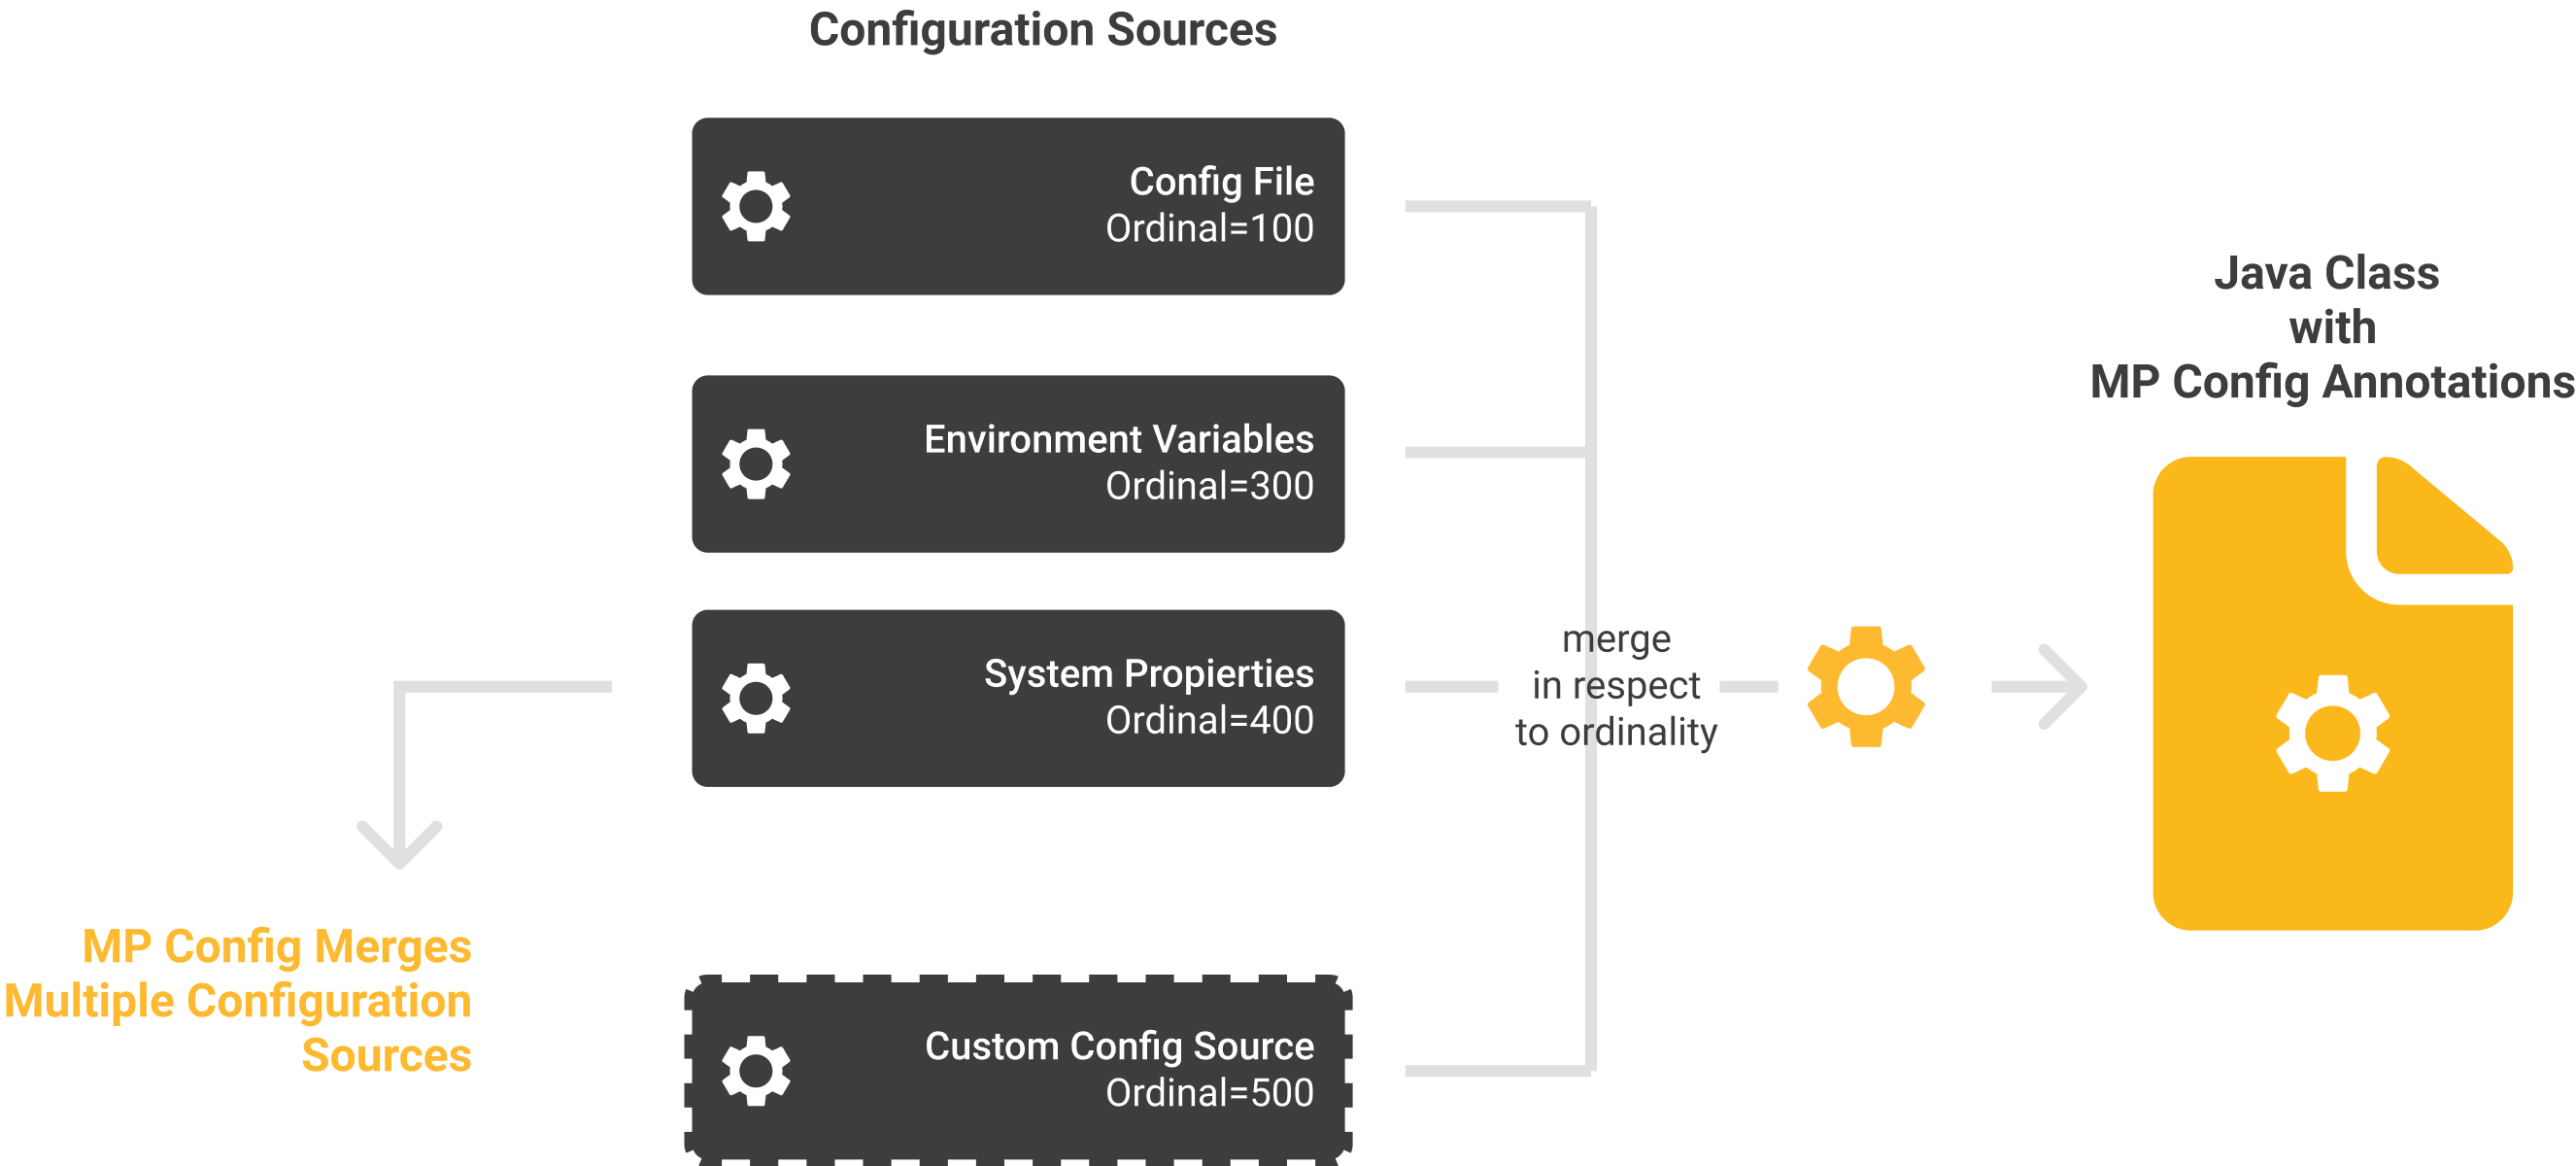
\includegraphics[width=0.8\linewidth]{Images/mpconfig}
\end{figure}
\end{frame}




\begin{frame}[fragile]{Config}
\begin{lstlisting}
@Inject
<@\textcolor{red}{@ConfigProperty(name = "omdbservice.url")}@>
String omdbDaemonServiceUrl;
\end{lstlisting}

Ext. da configuração(VM, Docker, Kubernetes)
\end{frame}



\begin{frame}[fragile]{Config}
\begin{lstlisting}
@Inject
@ConfigProperty(name = "application.currency")
private String currency;

@Inject
@ConfigProperty(name = "application.list.maxSize",
	defaultValue="10")
private Integer maxSize;
\end{lstlisting}
\end{frame}


\begin{frame}[fragile]{OpenAPI - REST}
Documentação padronizada
\begin{lstlisting}
@ApplicationPath("/api")
@OpenAPIDefinition(info = @Info(
	title = "Example application",
	version = "1.0.0",
	contact = @Contact(
	name = "Victor Orozoc",
	email = "vorozco@nabenik.com",
	url = "http://vorozco.com")
	),
	servers = {
		@Server(url = "/example",
		description = "localhost")
	}
)
public class ApplicationConfig extends Application {
\end{lstlisting}
\end{frame}

\begin{frame}[fragile]{OpenAPI}
Documentação padronizada
\begin{lstlisting}
@GET @Path("/{key}")
@Operation(description = "Get the value for this key")
@APIResponses({
	@APIResponse(responseCode = "200",
	description = "Successful, returning the value")
})
@Produces(MediaType.TEXT_PLAIN)
public Response getConfigValue(@PathParam("key") String key)
\end{lstlisting}
\end{frame}

\begin{frame}{OpenAPI}
\begin{figure}
	\centering
	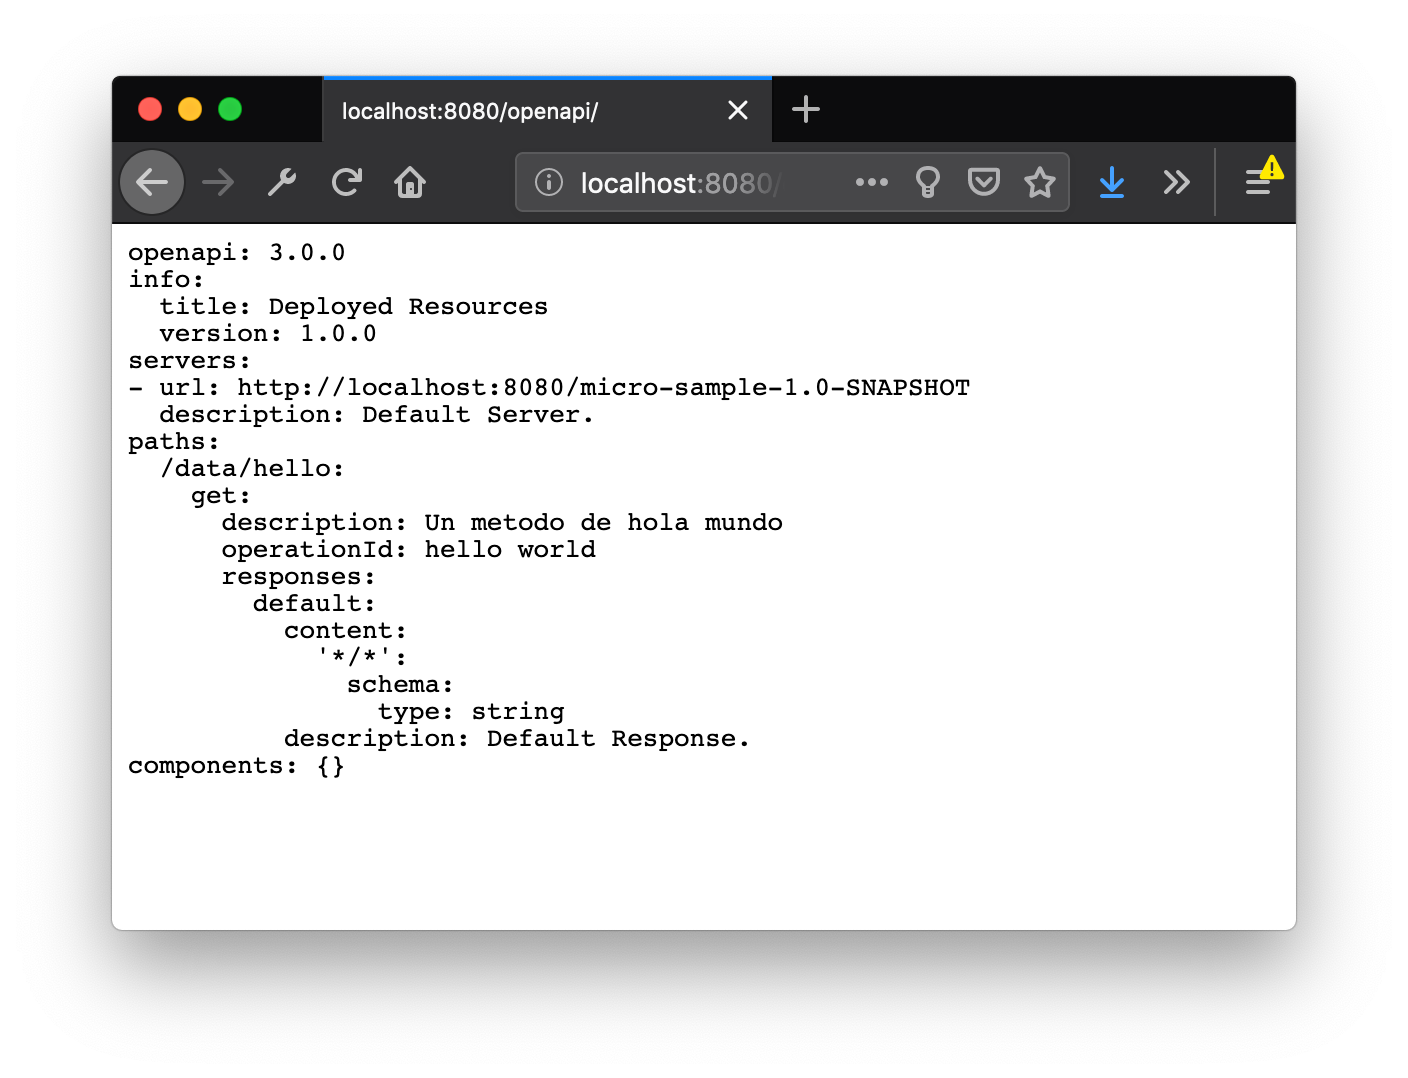
\includegraphics[width=0.75\linewidth]{Images/openapi}
\end{figure}
\end{frame}


\begin{frame}{Fault Tolerance}
\begin{figure}
	\centering
	
\includegraphics[width=0.75\linewidth]{Images/faulttolerance}
\end{figure}
\end{frame}

\begin{frame}{Metrics}
\begin{figure}
	\centering
	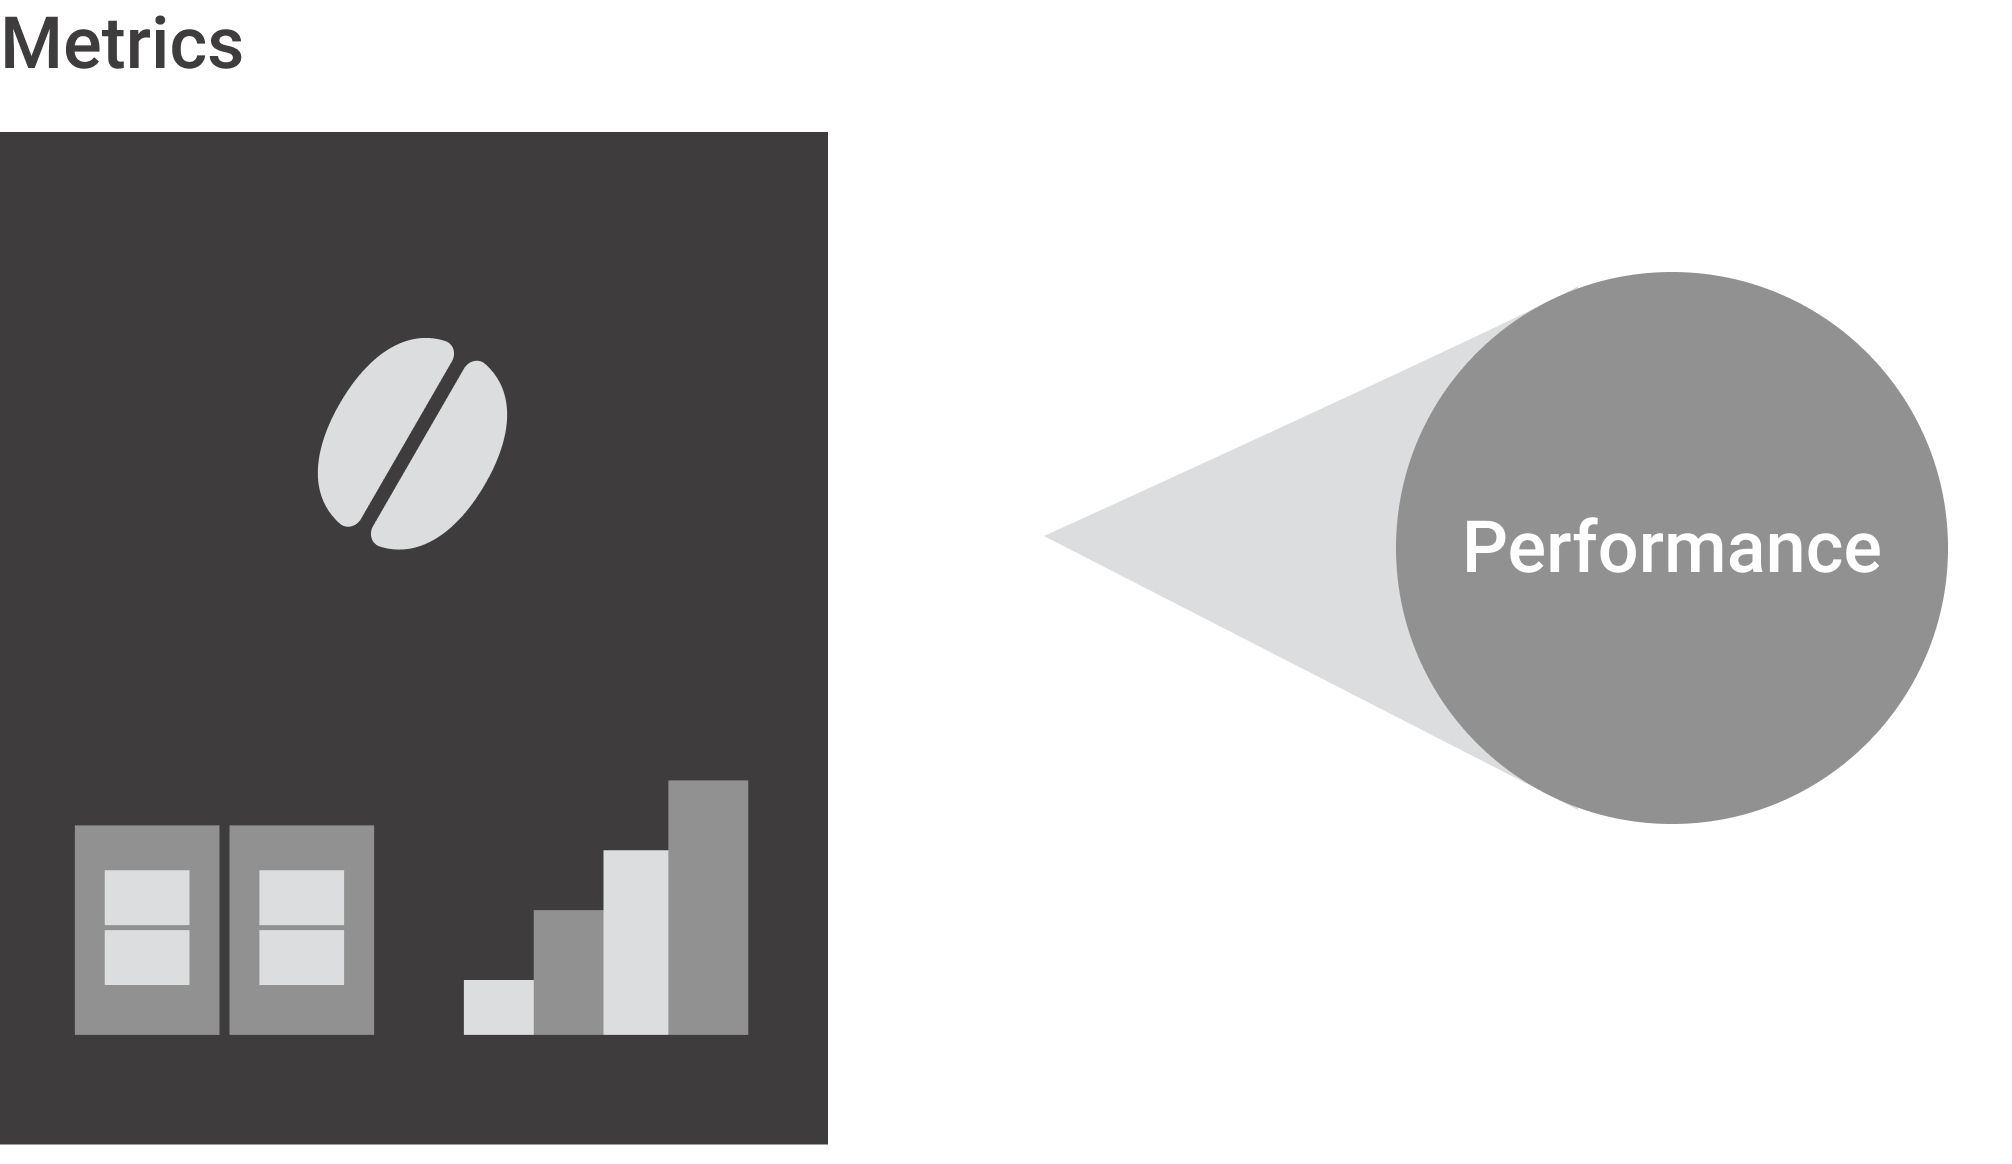
\includegraphics[width=0.75\linewidth]{Images/metrics}
\end{figure}
\end{frame}




\begin{frame}{Fault Tolerance + Metrics}

\begin{figure}
	\centering
	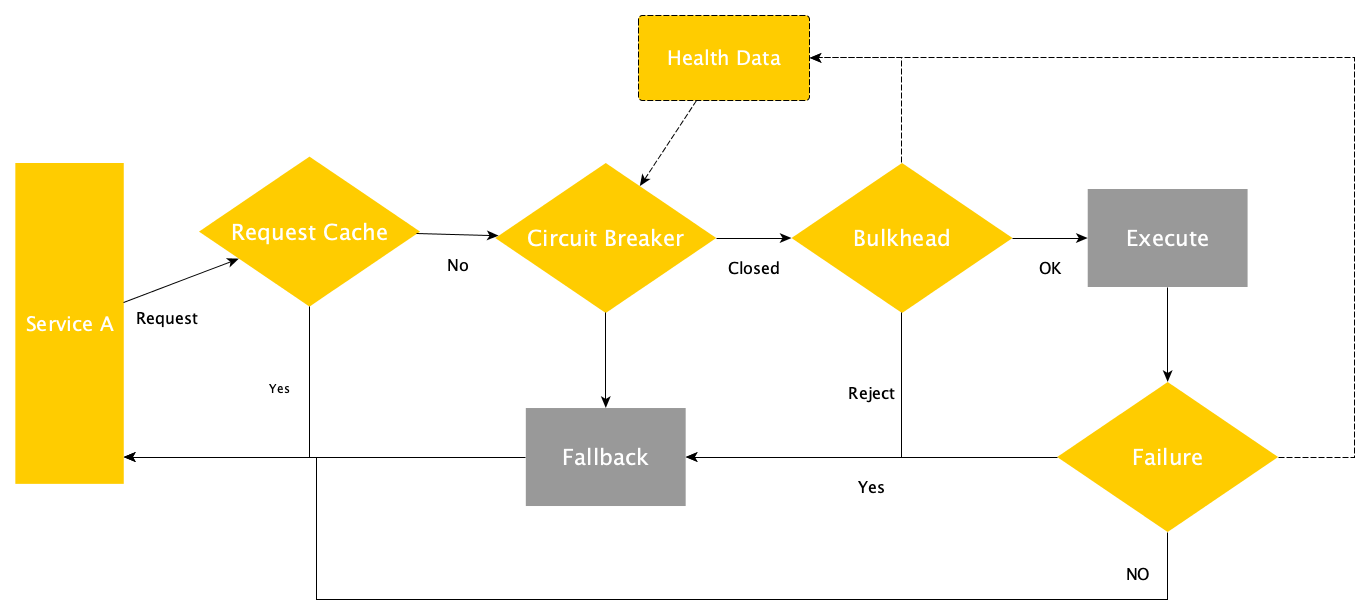
\includegraphics[width=0.9\linewidth]{Images/falldata}
\end{figure}

\end{frame}


\begin{frame}{Fault tolerance}
Regras e alternativas
\begin{itemize}
\item Circuit Breaker
\item Bulkhead
\item Retry
\item Timeout
\item Fallback
\end{itemize}

\end{frame}

\begin{frame}[fragile]{Fault tolerance - Retry}
\begin{lstlisting}
@Retry(delay = 400, maxDuration= 3200, jitter= 400, maxRetries = 10)
public Connection serviceA() {
	...
}

@Retry(retryOn = {IOException.class})
public void serviceB() {
	...
}
\end{lstlisting}
\end{frame}

\begin{frame}[fragile]{Fault tolerance - CircuitBreaker}
\begin{lstlisting}
@CircuitBreaker(successThreshold = 10,
	requestVolumeThreshold = 4,
	failureRatio=0.75,
	delay = 1000)
public Connection serviceA() {
	Connection conn = null;
	conn = connectionService();
	return conn;
}
\end{lstlisting}
\end{frame}

\begin{frame}[fragile]{Fault tolerance - Bulkhead}
\begin{lstlisting}
@Bulkhead(5)
public Connection serviceA() {
	Connection conn = null;
	conn = connectionService();
	return conn;
}
\end{lstlisting}

\begin{lstlisting}
@Asynchronous
@Bulkhead(value = 5, waitingTaskQueue = 8)
public Future<Connection> serviceA() {
	Connection conn = null;
	conn = connectionService();
	return CompletableFuture.completedFuture(conn);
}

\end{lstlisting}
\end{frame}



\begin{frame}[fragile]{Fault tolerance - Fallback, Timeout}
\begin{lstlisting}
@GET
@Path("/{id:[a-z]*[0-9][0-9]*}")
<@\textcolor{red}{@Fallback(fallbackMethod = "findByIdFallBack")}@>
<@\textcolor{red}{@Timeout(TIMEOUT)}@>
public Response findById(@PathParam("id")
final String imdbId) {
...
}

public Response findByIdFallBack(@PathParam("id")
final String imdbId) {
...
}
\end{lstlisting}
\end{frame}

\begin{frame}[fragile]{Fault tolerance - Fallback Handler, Timeout}
\begin{lstlisting}
@GET
@Path("/{id:[a-z]*[0-9][0-9]*}")
<@\textcolor{red}{@Fallback(MovieFindAllFallbackHandler.class)}@>
<@\textcolor{red}{@Timeout(TIMEOUT)}@>
public Response findById(@PathParam("id")
final String imdbId) {
...
}
\end{lstlisting}
\begin{lstlisting}
public class MovieFindAllFallbackHandler
	implements FallbackHandler<List> {
	@Override
	public List handle(final ExecutionContext context) {
		return Stream.of("Star Wars",
		"The Matrix", "Cantinflas").collect(toList());
	}
}
\end{lstlisting}
\end{frame}


\begin{frame}{Metrics}

\begin{itemize}
	\item JSON or OpenMetrics (Prometheus)
	\item Vendor
	\item Base
	\item Application
\end{itemize}

Opções
\begin{itemize}
	\item Counted
	\item Gauge
	\item Metered
	\item Timed
	\item Histogram
\end{itemize}

\end{frame}

\begin{frame}[fragile]{Metrics - Counted}
\begin{lstlisting}
@Inject
<@\textcolor{red}{@Metric}@>
Counter failedQueries;
\end{lstlisting}

\begin{lstlisting}
@GET
@Path("/{id:[a-z]*[0-9][0-9]*}")
<@\textcolor{red}{@Fallback(fallbackMethod = "findByIdFallBack")}@>
<@\textcolor{red}{@Timeout(TIMEOUT)}@>
public Response findById(@PathParam("id")
final String imdbId) {
...
}

public Response findByIdFallBack(@PathParam("id")
final String imdbId) {
	...
	<@\textcolor{red}{failedQueries.inc();}@>
}
\end{lstlisting}
\end{frame}

\begin{frame}[fragile]{Metrics - Gauge}
Inc-dec
\begin{lstlisting}
<@\textcolor{red}{
@Gauge(unit = "ExternalDatabases",
	name = "movieDatabases", absolute = true)
}@>
public long getDatabases() {
	return 99; //Any value
}
\end{lstlisting}

\lstinline|/metrics/application/movieDatabases|
\end{frame}

\begin{frame}[fragile]{Metrics - Metered}
Events rate
\begin{lstlisting}
@Metered(name = "moviesRetrieved",
	unit = MetricUnits.MINUTES,
	description = "Metrics to monitor movies",
	absolute = true)
public Response findExpandedById(
	@PathParam("id") final Long id)
\end{lstlisting}

\lstinline|/metrics/application/movieDatabases|
\end{frame}

\begin{frame}[fragile]{Metrics- Timed}
Performance
\begin{lstlisting}
@Timed(name = "moviesDelay",
	description = "Time to retrieve a movie",
	unit = MetricUnits.MINUTES,
	absolute = true)
public Response findExpandedById(
	@PathParam("id") final Long id)
\end{lstlisting}

\lstinline|/metrics/application/moviesDelay|
\end{frame}

\begin{frame}[fragile]{Metrics - Histogram}
Distribuciones
\begin{lstlisting}
@Inject
MetricRegistry registry;

@POST
@Path("/add/{attendees}")
public Response addAttendees(
	@PathParam("attendees") Long attendees) {
	Metadata metadata =
		new Metadata("matrix attendees",
			MetricType.HISTOGRAM);
	Histogram histogram =
		registry.histogram(metadata);
	histogram.update(attendees);
	return Response.ok().build();
}
\end{lstlisting}

\end{frame}

\begin{frame}{Health Check}
\begin{figure}
	\centering
	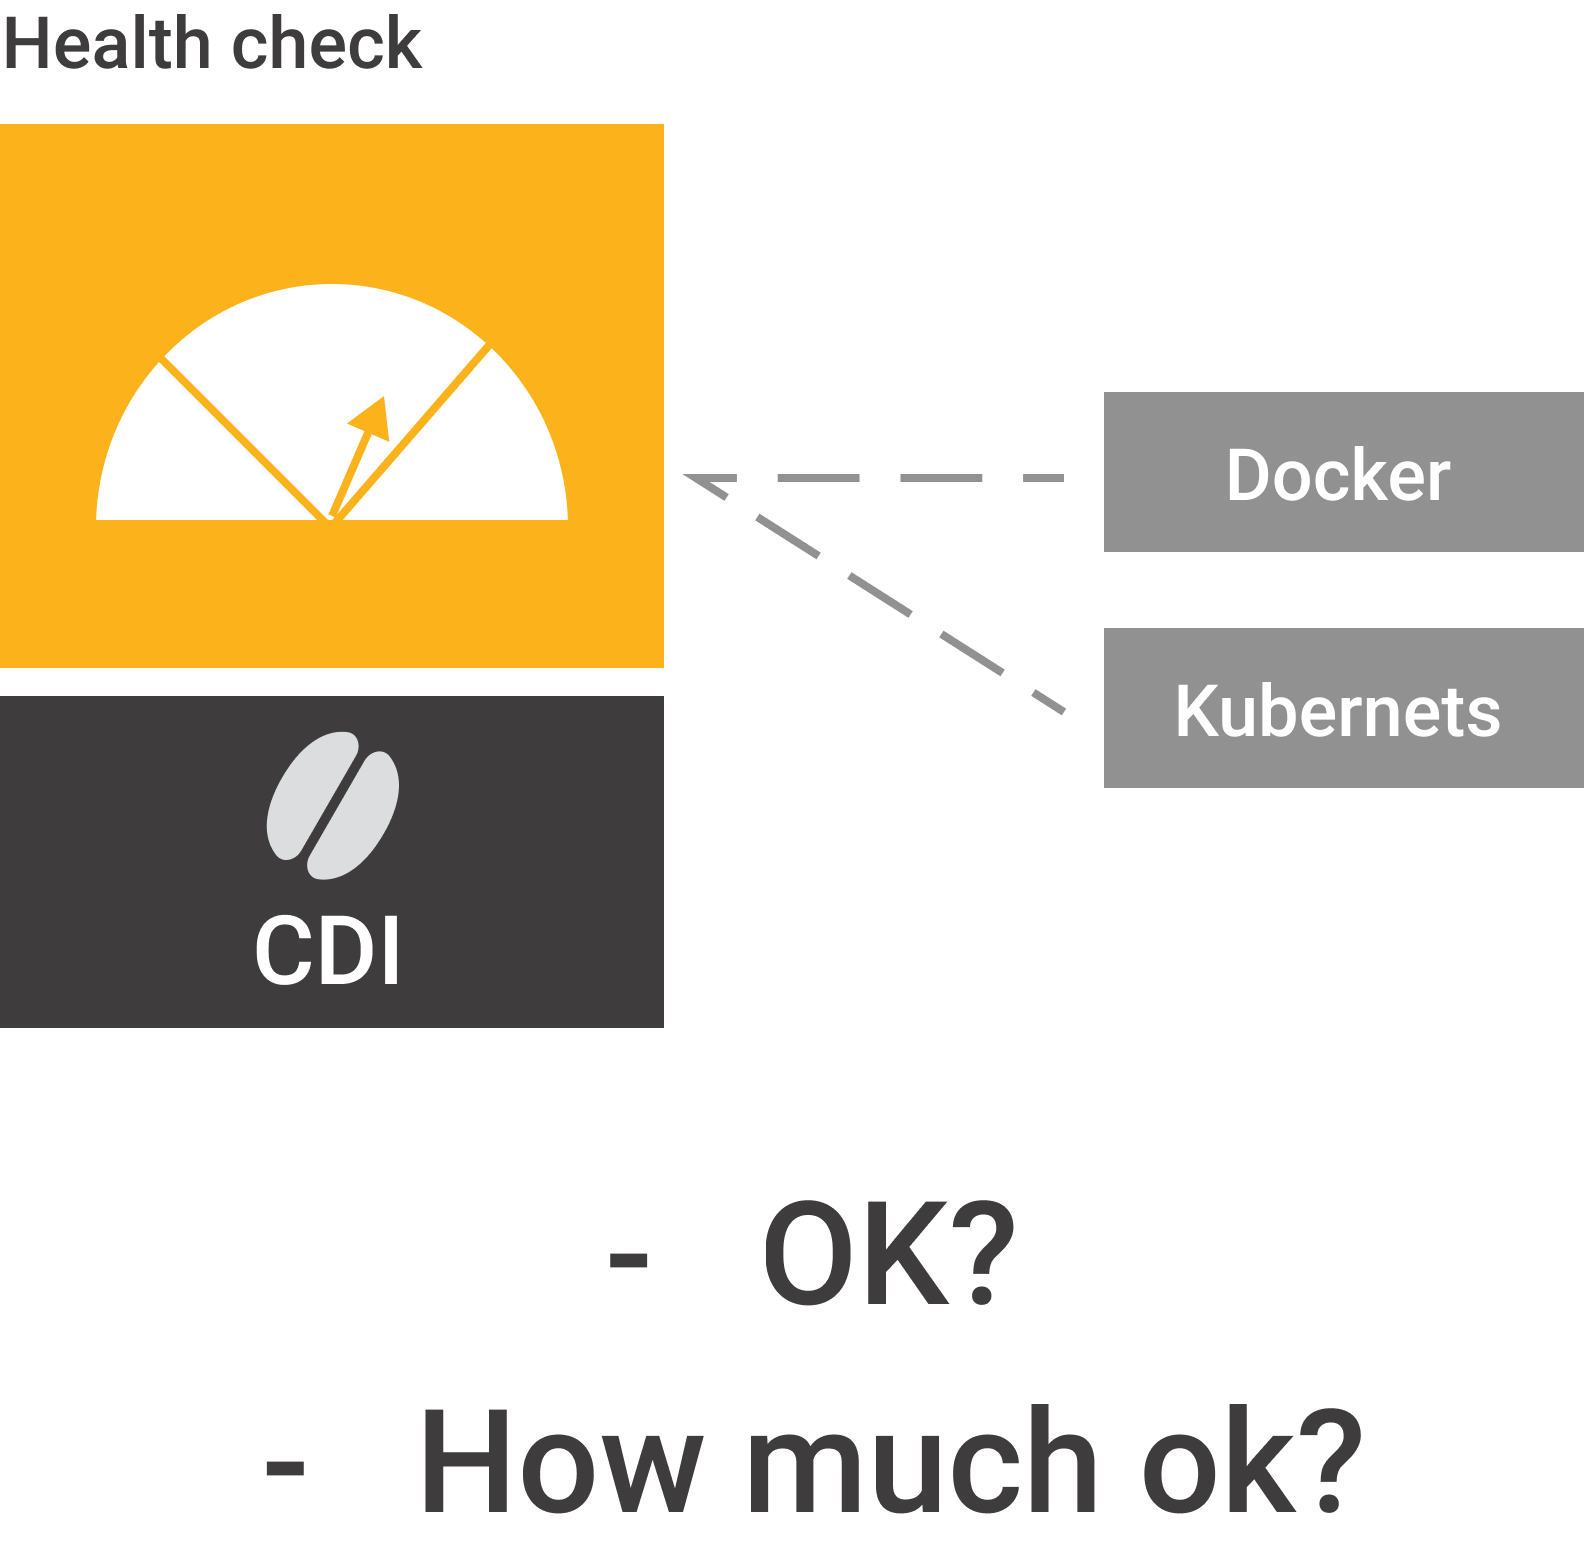
\includegraphics[width=0.75\linewidth]{Images/healthcheck}
\end{figure}
\end{frame}

\begin{frame}[fragile]{Health Check}
\begin{lstlisting}
@Override
public HealthCheckResponse call() {
	return HealthCheckResponse.named("TaVivoAinda")
		.withData("key1", "val1")
		.withData("key2", "val2")
		.up()
		.build();

}
\end{lstlisting}

\end{frame}


\begin{frame}{JWT}
\begin{figure}
	\centering
	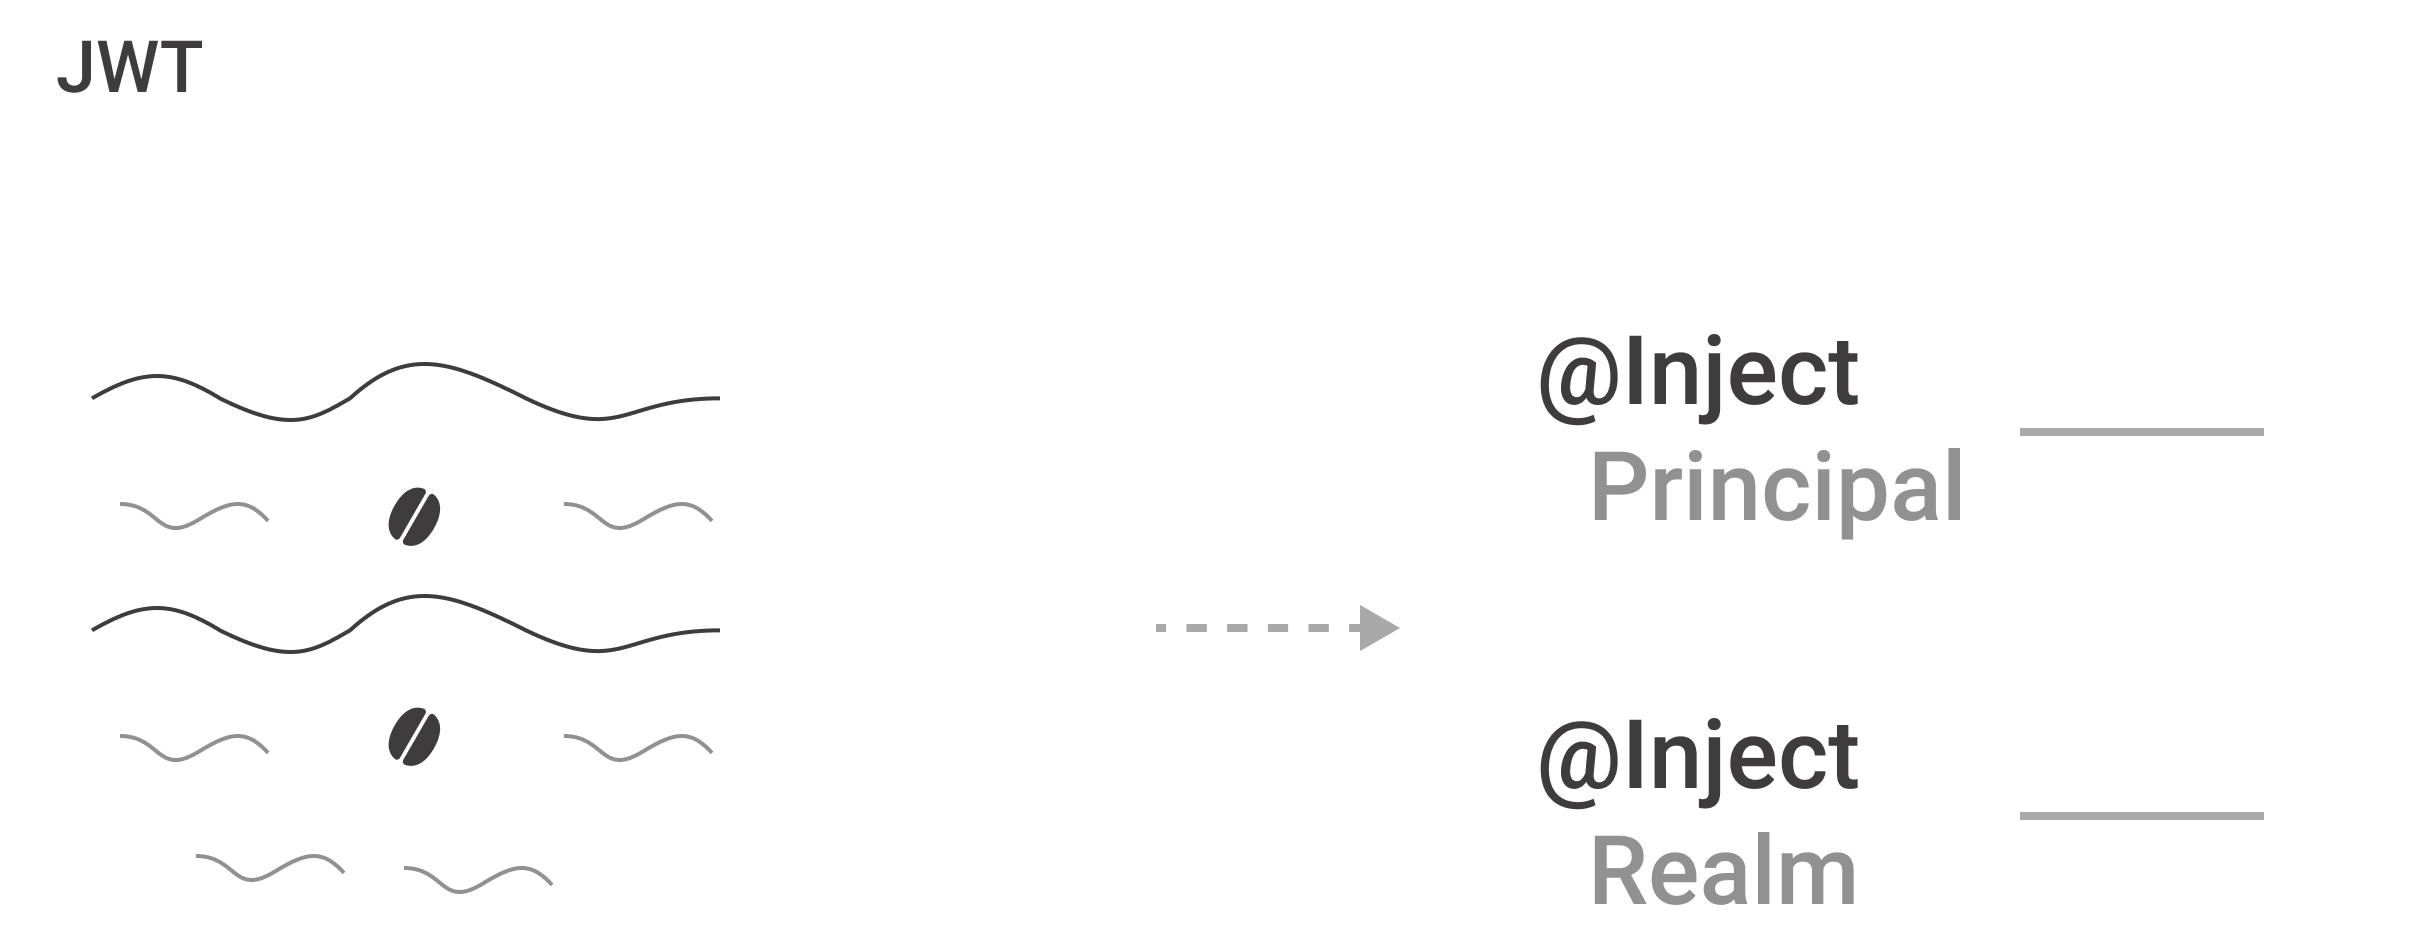
\includegraphics[width=0.9\linewidth]{Images/jwt}
\end{figure}
\end{frame}


\begin{frame}[fragile]{JWT}

\begin{lstlisting}
<@\textcolor{red}{@LoginConfig(authMethod = "MP-JWT")}@>
public class ApplicationConfig extends Application {
}
\end{lstlisting}

\begin{lstlisting}
@Inject
private JsonWebToken jwtPrincipal;

@Inject
<@\textcolor{red}{@Claim("email")}@>
private String email;
\end{lstlisting}
\end{frame}

\begin{frame}{TypeSafe}
\begin{figure}
	\centering
	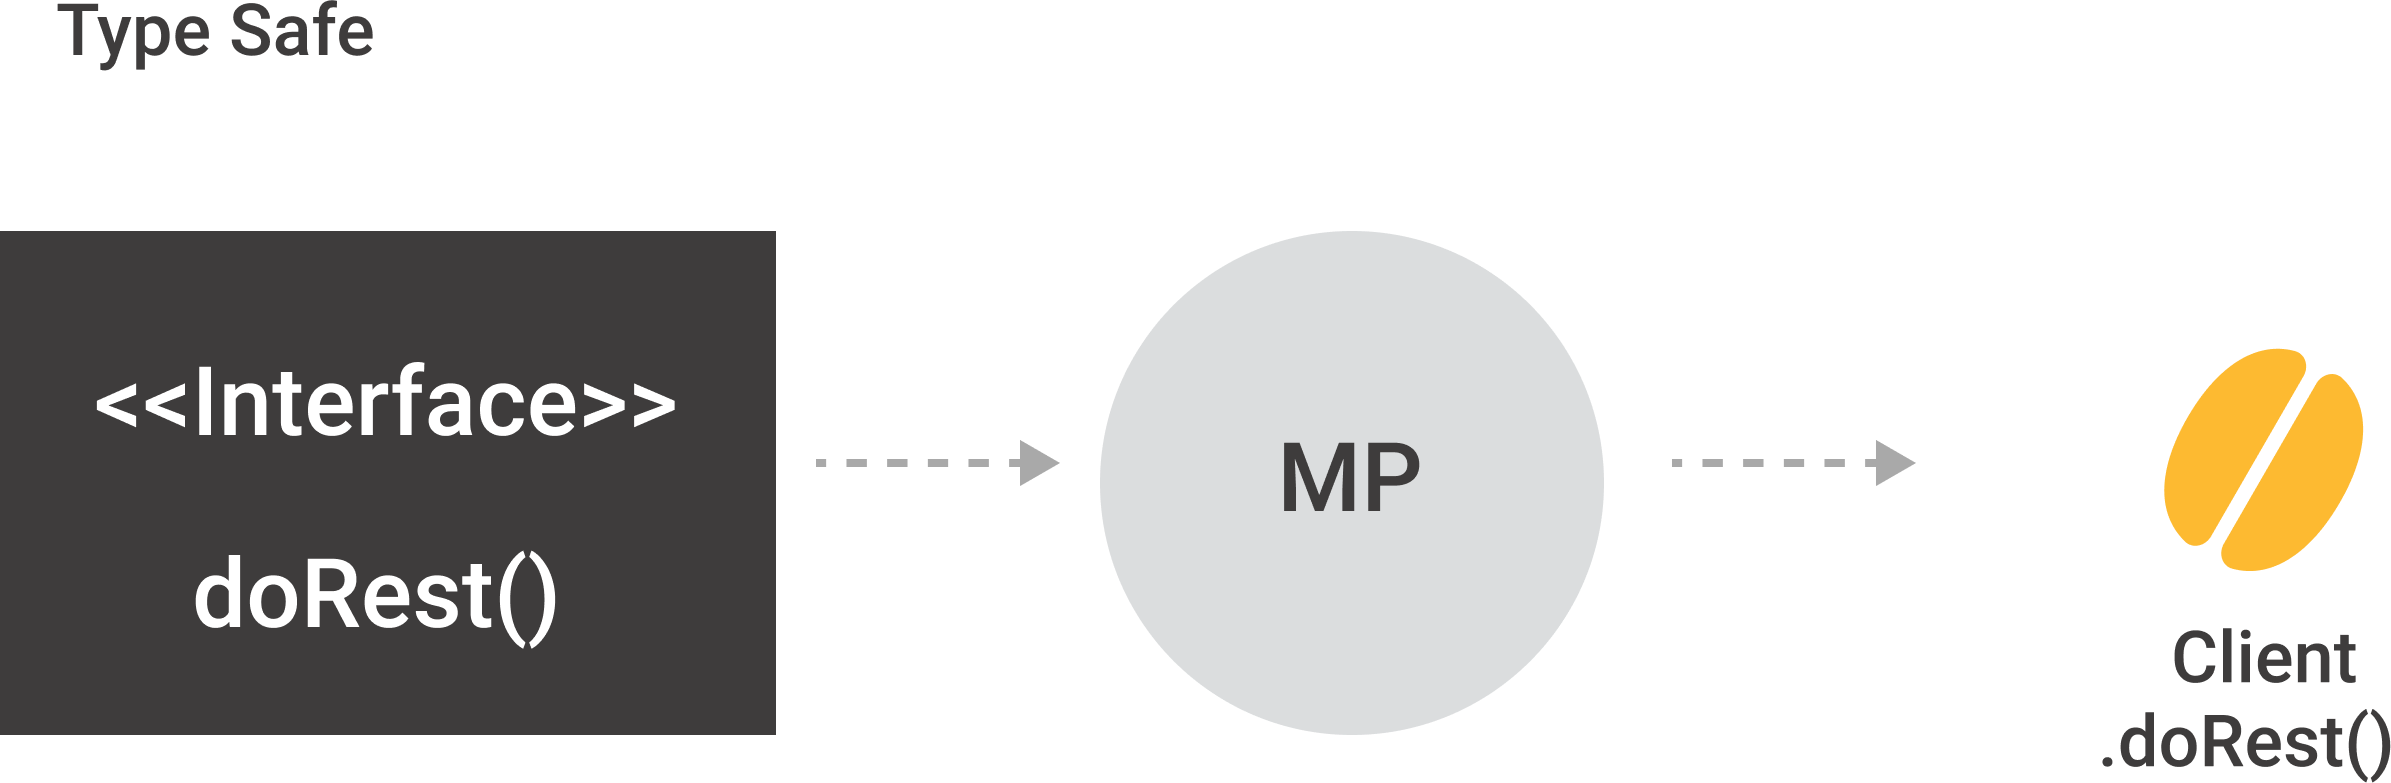
\includegraphics[width=0.75\linewidth]{Images/typesafe}
\end{figure}
\end{frame}

\begin{frame}[fragile]{TypeSafe}


\begin{lstlisting}
@Path("/playlist")
@Consumes("application/json")
public <@\textcolor{red}{interface}@> MusicPlaylistService {

	@GET
	List<String> getPlaylistNames();


	@PUT
	@Path("/{playlistName}")
	long updatePlayList(@PathParam("playlistName")
		String name,
		List<Song> playlist)
		throws UnknownPlaylistException;
}
\end{lstlisting}
\end{frame}


\begin{frame}{12 fatores cloud native (Heroku)}

\begin{columns}[T] % contents are top vertically aligned

	\begin{column}[T]{4cm} % alternative top-align that's better for graphics
		\begin{alertblock}{Microprofile}
	\begin{itemize}
		\item Config
		\item Backing service
		\item Disposability
	\end{itemize}
\end{alertblock}
	\end{column}
	\begin{column}[T]{6cm} % each column can also be its own environment
		\begin{block}{Cloud}
	\begin{itemize}
	\item Codebase (Git-Flow)
	\item Dependencies (Maven)
	\item Build, Release, Run
	\item Processes (Pipelines)
	\item Port binding
	\item Concurrency (Docker - k8s)
	\item Dev / Prod parity
	\item Logs
	\item Admin process
\end{itemize}
\end{block}
	\end{column}
\end{columns}

\end{frame}



\begin{frame}{Víctor Orozco}
    \begin{columns}[T] % contents are top vertically aligned

        \begin{column}[T]{4cm} % alternative top-align that's better for graphics
            \begin{figure}
                \centering
                
\includegraphics[width=\linewidth]{Images/logos}
            \end{figure}
        \end{column}
        \begin{column}[T]{6cm} % each column can also be its own environment
            \begin{itemize}
                \item vorozco@nabenik.com
                \item \href{https://twitter.com/tuxtor}{@tuxtor}
                \item \href{http://vorozco.com}{http://vorozco.com}
                \item \href{http://tuxtor.shekalug.org}{http://tuxtor.shekalug.org}
            \end{itemize}
            \begin{center}
                
\includegraphics[width=0.1\linewidth]{Images/cclogo}
                \\
                This work is licensed under Creative Commons Attribution-NonCommercial-ShareAlike 3.0 Guatemala (CC BY-NC-SA 3.0 GT).
            \end{center}
        \end{column}
    \end{columns}
\end{frame}



\end{document}
